\def\type{problem}

\begin{problem}[1]
  Find all the solutions of $\sin(z) = i$.
\end{problem}

\begin{solution}
  Using the complex exponential form of the sine function, we have
  \[%
    \sin(z) = \frac{e^{iz} - e^{-iz}}{2i} = i
  .\]%
  Multiplying both sides by $2i$ gives $e^{iz} - e^{-iz} = -2$. Let $w = e^{iz}$, then we get the quadratic $w^2 + 2w - 1 = 0$. Using the quadratic formula, we find $w = -1 \pm \sqrt{2}$. Since $w = e^{iz}$, taking logarithms gives and multiplying by $-i$ gives $z = -i \ln(w)$, giving us two branches of solutions, $-1 + \sqrt{2}$ and $-1 - \sqrt{2}$.

  For the first branch, $w = -1 + \sqrt{2} > 0$, we get $\arg(w) = 0$. So
  \[%
    \ln(w) = \ln\left(-1 + \sqrt{2}\right) + 2\pi i k
  ,\]%
  and
  \[%
    z = -i\ln\left(-1 + \sqrt{2}\right) + 2\pi k, \quad k \in \Z
  .\]%

  For the second branch, $w = -1 - \sqrt{2} < 0$, we get $\arg(w) = \pi$. So
  \[%
    \ln(w) = \ln\left(-1 - \sqrt{2}\right) + i\pi + 2\pi i k
  ,\]%
  and
  \[%
    z = -i\ln\left(-1 - \sqrt{2}\right) + \pi + 2\pi k, \quad k \in \Z
  .\]%

  Therefore, the complete set of solutions is
  \[%
    z = -i\ln\left(-1 + \sqrt{2}\right) + 2\pi k \oor z = -i\ln\left(-1 - \sqrt{2}\right) + \pi + 2\pi k, \quad k \in \Z
  .\qedhere\]%
\end{solution}

\begin{problem}[2]
  Let $\gamma_0$ be the path which consists of line segments from $-1$ to $i$ and then from $i$ to $1$. Let $\gamma_1$ be the path which consists of line segments from $-1$ to $-i$ and then from $-i$ to $1$. Evaluate the following two integrals
  \[%
    \int_{\gamma_0} z^{-1} \dz; \quad \int_{\gamma_1} z^{-1} \dz
  .\]%
\end{problem}

\begin{solution}
  Graphing the contour paths, we have
  \begin{figure}[H]
    \centering

    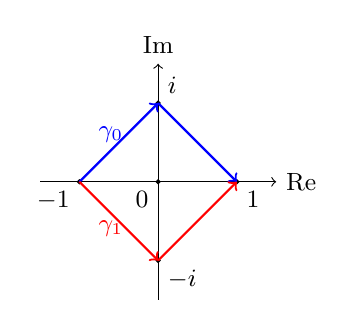
\begin{tikzpicture}

      % Axes
      \draw[->] (-1.5,0) -- (1.5,0) node[right] {\small Re};
      \draw[->] (0,-1.5) -- (0,1.5) node[above] {\small Im};

      % Points
      \filldraw (-1,0) circle (0.7pt) node[below left] {\small $-1$};
      \filldraw (1,0) circle (0.7pt) node[below right] {\small $1$};
      \filldraw (0,1) circle (0.7pt) node[above right] {\small $i$};
      \filldraw (0,-1) circle (0.7pt) node[below right] {\small $-i$};
      \filldraw (0,0) circle (0.7pt) node[below left] {\small $0$};

      % Path gamma_0: -1 to i to 1 (counterclockwise)
      \draw[thick, blue, ->] (-1,0) -- (0,1);
      \draw[thick, blue, ->] (0,1) -- (1,0);
      \node[blue] at (-0.6,0.6) {\small $\gamma_0$};

      % Path gamma_1: -1 to -i to 1 (clockwise)
      \draw[thick, red, ->] (-1,0) -- (0,-1);
      \draw[thick, red, ->] (0,-1) -- (1,0);
      \node[red] at (-0.6,-0.6) {\small $\gamma_1$};
    \end{tikzpicture}
  \end{figure}

  The integrand is $f(z) = \sfrac{1}{z}$, which has a simple pole at $z = 0$. The value of the contour integral of $\sfrac{1}{z}$ depends on whether the path encloses the origin and in which direction.

  The path $\gamma_0$ consists of the segments from $-1$ to $i$ and then $i$ to $1$. Together, they form a triangle that encloses the origin in the counterclockwise direction. Since $\sfrac{1}{z}$ is holomorphic everywhere on and inside the path except at the singularity $z = 0$, and the path encloses the singularity once counterclockwise, it follows from Cauchy's theorem that
  \[%
    \int_{\gamma_0} \frac{1}{z} \dz = 2\pi i
  .\]%

  Similarly, the path $\gamma_1$ consists of the segments from $-1$ to $-i$ and then $-i$ to $1$, which also enclose the origin, but now in the **clockwise** direction. Therefore, we get
  \[%
    \int_{\gamma_1} \frac{1}{z} \dz = -2\pi i
  .\]%

  Therefore, we have
  \[%
    \int_{\gamma_0} \frac{1}{z} \dz = 2\pi i \aand \int_{\gamma_1} \frac{1}{z} \dz = -2\pi i
  .\qedhere\]%
\end{solution}

\begin{problem}[3]
  Let $C_r = \{z \mid \abs{z} = r\}$, for $0 < r \ne 2$ your answer might depend on $r$). Find the integral
  \[%
    \int_{C_r} \frac{1}{z^3 - 2z^2} \dz
  .\]%
\end{problem}

\begin{solution}
  We begin by factoring the denominator to get
  \[%
    \frac{1}{z^3 - 2z^2} = \frac{1}{z^2(z - 2)}
  .\]%
  The integrand has singularities at $z = 0$ (a pole of order 2) and $z = 2$ (a simple pole). The integral depends on the location of these singularities relative to the contour $C_r$. In the case where $0 < r < 2$, $C_r$ encloses the singularity at $z = 0$, but not $z = 2$. Since the integrand is holomorphic on and inside $C_r$ except at $z = 0$, we compute the residue at $z = 0$. Expanding using partial fraction decomposition, we have
  \[%
    f(z) = \frac{1}{z^2(z - 2)} = \frac{A}{z - 2} + \frac{B}{z} + \frac{C}{z^2}
  ,\]%
  for constants $A, B, C$. Multiply both sides by $z^2(z - 2)$ and solve to get
  \[%
    1 = A z^2 + B z(z - 2) + C(z - 2)
  .\]%
  Then, expand and collect terms to get
  \[%
    1 = Az^2 + Bz^2 - 2Bz + Cz - 2C = (A + B)z^2 + (C - 2B)z - 2C
  .\]%
  By comparing and solving for the coefficients, we have
  \[%
    A = \frac{1}{4}, \quad B = -\frac{1}{4}, \aand C = -\frac{1}{2}
  .\]%
  So,
  \[%
    \frac{1}{z^2(z - 2)} = \frac{1}{4(z - 2)} - \frac{1}{4z} - \frac{1}{2z^2}
  .\]%
  On the circle $C_r$ with $r < 2$, only the terms with singularities at $z = 0$ contribute to the integral. The term $\sfrac{1}{4(z - 2)}$ is analytic inside $C_r$, so its integral is $0$. We compute
  \[%
    \int_{C_r} \frac{1}{z^2(z - 2)} \dz = \int_{C_r} \left(-\frac{1}{4z} - \frac{1}{2z^2}\right) \dz = -\frac{1}{4} \int_{C_r} \frac{1}{z} \dz - \frac{1}{2} \int_{C_r} \frac{1}{z^2} \dz
  .\]%
  Now, by Cauchy's integral formula, we have
  \[%
    \int_{C_r} \frac{1}{z^2(z - 2)} \dz = -\frac{1}{4} (2\pi i) = -\frac{\pi i}{2}
  .\]%

  In the case where $r > 2$, both $z = 0$ and $z = 2$ lie inside $C_r$, so all three terms contribute, giving us
  \[
    \int_{C_r} \frac{1}{z^2(z - 2)} \dz = \int_{C_r} \left(\frac{1}{4(z - 2)} - \frac{1}{4z} - \frac{1}{2z^2}\right) \dz = \frac{1}{4}(2\pi i) - \frac{1}{4}(2\pi i) - 0 = 0
  .\]%

  Therefore, we conclude that
  \[%
    \int_{C_r} \frac{1}{z^3 - 2z^2} \dz = \begin{cases}
      -\dfrac{\pi i}{2} & \text{if}~0 < r < 2 \\
      0 & \text{if}~r > 2 \\
    \end{cases}
  .\qedhere\]%
\end{solution}

\begin{problem}[4]
  Let $f$ be an entire function such that $\lim_{z \to \infty} f(z) z^{-2} = 0$. Use Cauchy’s integral formula to show that $f''(z) = 0$ for any $z$, hence $f(z) = az + b$ for some constants $a, b \in \C$.
\end{problem}

\begin{solution}
  Since $f$ is entire, it is holomorphic on all of $\C$. Fix any $z \in \C$ and let $R > 0$ be large enough so that $z$ lies inside the disk $D(0, R)$. Then, by Cauchy's integral formula for the second derivative, we have
  \[%
    f''(z) = \frac{2!}{2\pi i} \int_{\abs{\zeta} = R} \frac{f(\zeta)}{(\zeta - z)^3} \dd{\zeta}
  .\]%
  Since $\abs{\zeta - z} \geq \abs{\zeta} - \abs{z} = R - \abs{z}$ for $\abs{\zeta} = R$, and since $f$ is entire with the property that $\lim_{\zeta \to \infty} \frac{f(\zeta)}{\zeta^2} = 0$, we can write
  \[%
    \abs{f(\zeta)} \leq \epsilon \abs{\zeta}^2 = \epsilon R^2, \quad \text{for all}~\abs{\zeta} = R~\text{with $R$ sufficiently large}
  ,\]%
  for any $\epsilon > 0$. Thus, we estimate
  \[%
    \abs{f''(z)} \leq \frac{2}{2\pi} \int_{\abs{\zeta} = R} \frac{\abs{f(\zeta)}}{\abs{\zeta - z}^3} \abs{\dd{\zeta}} \leq \frac{2}{2\pi} \cdot \frac{\epsilon R^2}{(R - \abs{z})^3} \cdot 2\pi R = \frac{2\epsilon R^3}{(R - \abs{z})^3}
  .\]%
  Now, taking the limit as $R \to \infty$, we note that the right-hand side tends to $0$:
  \[%
    \lim_{R \to \infty} \frac{2\epsilon R^3}{(R - \abs{z})^3} = 2\epsilon
  .\]%
  Since $\epsilon > 0$ was arbitrary, we conclude that $\abs{f''(z)} = 0$, so $f''(z) = 0$ for all $z \in \C$.

  Therefore, $f$ is a polynomial of degree at most $1$, so there exist constants $a, b \in \C$ such that
  \[%
    f(z) = az + b
  .\qedhere\]%
\end{solution}

\begin{problem}[5]
  Let $f$ be an entire function such that $\abs{f(z)} \ge 1$ and $f(0) = i$. Prove that $f(z) = i$ for all $z$.
\end{problem}

\begin{solution}
  Since $f$ is entire, it is holomorphic on all of $\C$. Moreover, the condition $\abs{f(z)} \ge 1$ for all $z \in \C$ implies that the function $f$ never vanishes, so we may define the function
  \[%
    g(z) = \frac{1}{f(z)}
  ,\]%
  for all $z \in \C$. Then $g$ is entire, since the reciprocal of a non-vanishing holomorphic function is holomorphic.

  Furthermore, for all $z \in \C$, we have
  \[%
    \abs{g(z)} = \abs{\frac{1}{f(z)}} \le \frac{1}{1} = 1
  ,\]%
  so $g$ is a bounded entire function. By Liouville’s theorem in Sec. 53, $g$ is constant. Hence, $f(z)$ is constant as well.

  Since $f(0) = i$, we conclude that
  \[%
    f(z) = i \quad \text{for all } z \in \C
  .\qedhere\]%
\end{solution}

\begin{problem}[6]
  Compute (use contour integral)
  \[%
    \int_0^\infty \frac{1}{1 + x^6} \dx
  .\]%
\end{problem}

\begin{solution}
  We begin by observing that the integrand is an even function, so we can extend the domain of integration to the entire real line and halve the result, i.e.,
  \[%
    \int_0^\infty \frac{1}{1 + x^6} \dx = \frac{1}{2} \int_{-\infty}^\infty \frac{1}{1 + x^6} \dx
  .\]%
  We evaluate the full integral using contour integration. Let
  \[%
    f(z) = \frac{1}{1 + z^6}
  ,\]%
  and integrate this function over the semicircular contour in the upper half-plane of radius $R$, consisting of the real interval $[-R, R]$ and the semicircular arc $\gamma_R$ in the upper half-plane. As $R \to \infty$, the integral over $\gamma_R$ vanishes, so the integral over the real axis is given by the sum of the residues inside the contour.

  The function $f(z)$ has poles at the sixth roots of $-1$, that is, at
  \[%
    z_k = e^{i(2k+1)\sfrac{\pi}{6}}, \quad k = 0, 1, 2, 3, 4, 5
  .\]%
  The three poles in the upper half-plane are
  \[%
    z_0 = e^{i\sfrac{\pi}{6}}, \quad z_1 = e^{i\sfrac{\pi}{2}}, \aand z_2 = e^{i5\sfrac{\pi}{6}}
  .\]%

  These are all simple poles, and we compute the residue at each using the formula
  \[%
    \Res_{z = z_k} \left(\frac{1}{1 + z^6}\right) = \frac{1}{6z_k^5}
  .\]%
  Thus, the integral over the real line is
  \[%
    \int_{-\infty}^\infty \frac{1}{1 + x^6} \dx = 2\pi i \sum_{k=0}^2 \Res_{z = z_k} f(z) = 2\pi i \cdot \frac{1}{6} \left(\frac{1}{z_0^5} + \frac{1}{z_1^5} + \frac{1}{z_2^5}\right)
  .\]%

  We compute each of the terms to get
  \begin{alignat*}{5}
    z_0^5 &= e^{i5\sfrac{\pi}{6}} &&\implies \frac{1}{z_0^5} &&= e^{-i5\sfrac{\pi}{6}} \\
    z_1^5 &= e^{i5\sfrac{\pi}{2}} = e^{i\pi/2} &&\implies \frac{1}{z_1^5} &&= e^{-i\sfrac{\pi}{2}} \\
    z_2^5 &= e^{i25\sfrac{\pi}{6}} = e^{i\pi/6} &&\implies \frac{1}{z_2^5} &&= e^{-i\sfrac{\pi}{6}}
  .\end{alignat*}

  Therefore,
  \[%
    \int_{-\infty}^\infty \frac{1}{1 + x^6} \dx = 2\pi i \cdot \frac{1}{6} \left(e^{-i5\pi/6} + e^{-i\pi/2} + e^{-i\pi/6}\right)
  .\]%
  Compute the sum of exponentials to get
  \begin{align*}
    e^{-i5\sfrac{\pi}{6}} &= -\frac{\sqrt{3}}{2} - \frac{1}{2}i \\
    e^{-i\sfrac{\pi}{2}}  &= -i \\
    e^{-i\sfrac{\pi}{6}}  &= \frac{\sqrt{3}}{2} - \frac{1}{2}i
  ,\end{align*}
  and summing,
  \[%
    e^{-i5\sfrac{\pi}{6}} + e^{-i\sfrac{\pi}{2}} + e^{-i\sfrac{\pi}{6}} = \left(-\frac{\sqrt{3}}{2} + \frac{\sqrt{3}}{2}\right) + \left(-\frac{1}{2} - 1 - \frac{1}{2}\right)i = -2i
  .\]%

  Substituting into the integral,
  \[%
    \int_{-\infty}^\infty \frac{1}{1 + x^6} \dx = 2\pi i \cdot \frac{-2i}{6} = \frac{4\pi}{6} = \frac{2\pi}{3}
  .\]%

  Finally, since our original integral was half of this,
  \[%
    \int_0^\infty \frac{1}{1 + x^6} \dx = \frac{1}{2} \cdot \frac{2\pi}{3} = \frac{\pi}{3}
  .\qedhere\]%
\end{solution}

\begin{problem}[7]
  Compute (use contour integral)
  \[%
    \int_0^{2\pi} \frac{1}{2 + \cos(t)} \dt
  .\]%
\end{problem}

\begin{solution}
  We begin by transforming the integral using the complex exponential substitution $z = e^{it}$, which maps the interval $t \in [0, 2\pi]$ onto the unit circle $|z| = 1$ traversed once counterclockwise. Recall the identities
  \[%
    \cos(t) = \frac{1}{2}(e^{it} + e^{-it}) = \frac{1}{2}\left(z + \frac{1}{z}\right) \implies \dt = \frac{\dz}{iz}
  .\]%
  Substituting into the integrand, we have
  \[%
    \frac{1}{2 + \cos t} = \frac{1}{2 + \frac{1}{2}(z + z^{-1})} = \frac{2}{4 + z + z^{-1}}
  .\]%
  Therefore, the integral becomes
  \[%
    \int_0^{2\pi} \frac{1}{2 + \cos t} \dt = \oint_{|z|=1} \frac{2}{4 + z + \frac{1}{z}} \cdot \frac{1}{iz} \dz
  .\]%
  Combining terms gives us
  \[%
    \frac{2}{i z \left(4 + z + \frac{1}{z}\right)} = \frac{2}{i \left(z^2 + 4z + 1\right)}
  .\]%
  Thus, the integral reduces to:
  \[%
    \oint_{\abs{z}=1} \frac{2}{i(z^2 + 4z + 1)} \dz
  .\]%

  Now, we can evaluate this integral using the Residue theorem. The integrand has simple poles at the roots of the denominator, which are
  \[%
    z^2 + 4z + 1 = 0 \implies z = -2 \pm \sqrt{3}
  .\]%
  Only one of these poles lies within the unit circle, since $z_0 = -2 + \sqrt{3} \approx -0.2679$, since $\abs{-2 + \sqrt{3}} < 1$. We compute the residue of the integrand at $z_0$. For a simple pole, the residue is given by
  \[%
    \Res_{z=z_0} \left(\frac{2}{i(z^2 + 4z + 1)}\right) = \frac{2}{i} \cdot \frac{1}{(z_0 - z_1)}
  ,\]%
  where $z_1 = -2 - \sqrt{3}$ is the other root. Hence,
  \[%
    z_0 - z_1 = 2\sqrt{3} \implies \Res_{z=z_0} = \frac{2}{i \cdot 2\sqrt{3}} = \frac{1}{i \sqrt{3}} = -\frac{i}{\sqrt{3}}
  .\]%
  Therefore, by the Residue theorem, we have
  \[%
    \oint_{|z|=1} \frac{2}{i(z^2 + 4z + 1)} \dz = 2\pi i \cdot \left(-\frac{i}{\sqrt{3}}\right) = \frac{2\pi}{\sqrt{3}}
  .\]%

  Finally, we conclude that
  \[%
    \int_0^{2\pi} \frac{1}{2 + \cos(t)} \dt = \frac{2\pi}{\sqrt{3}}
  .\qedhere\]%
\end{solution}

\begin{problem}[8]
  Find the Taylor series of $f(z) = \sfrac{3}{(3 + z)^2}$ at $z = 0$. What is its convergence radius?
\end{problem}

\begin{solution}
  We begin by rewriting the function in a form suitable for expansion as a binomial series. Observe that
  \[%
    f(z) = \frac{3}{(3 + z)^2} = \frac{3}{9 \left(1 + \frac{z}{3}\right)^2} = \frac{1}{3} \cdot \left(1 + \frac{z}{3}\right)^{-2}
  .\]%
  Now we apply the generalized binomial series
  \[%
    (1 + w)^\alpha = \sum_{n=0}^\infty \binom{\alpha}{n} w^n, \quad \text{for}~\abs{w} < 1
  ,\]%
  with $\alpha = -2$ and $w = \sfrac{z}{3}$. We compute
  \[%
    \left(1 + \frac{z}{3}\right)^{-2} = \sum_{n=0}^\infty \binom{-2}{n} \left( \frac{z}{3} \right)^n
  .\]%
  Using the identity
  \[%
    \binom{-2}{n} = (-1)^n \binom{n + 1}{1} = (-1)^n (n + 1)
  ,\]%
  we obtain
  \[%
    f(z) = \frac{1}{3} \sum_{n=0}^\infty (-1)^n (n+1) \left( \frac{z}{3} \right)^n = \sum_{n=0}^\infty (-1)^n \frac{n+1}{3^{n+1}} z^n
  .\]%

  To determine the radius of convergence, we locate the nearest singularity of the function $f(z) = \sfrac{3}{(3 + z)^2}$. The only singularity is at $z = -3$, so the distance from the origin is $R = \abs{-3} = 3$.

  Hence, we get
  \[%
    f(z) = \sum_{n=0}^\infty (-1)^n \frac{n+1}{3^{n+1}} z^n \aand R = 3
  .\qedhere\]%
\end{solution}
